\documentclass[11pt]{article}
\usepackage{graphicx}
\usepackage{hyperref}
%\usepackage{appendix}
\usepackage{amsmath}
\usepackage{amsthm}
\usepackage{amssymb}
\usepackage{float}
\usepackage{commath}
%\usepackage{siunitx}
%\sisetup{detect-all}
\usepackage[a4paper,margin=20mm]{geometry}
\numberwithin{equation}{section}
\setlength{\parskip}{\baselineskip}
\setlength{\parindent}{0pt}
\hypersetup{
    colorlinks=true,
    linkcolor=magenta,
    filecolor=magenta,      
    urlcolor=magenta,
}
\urlstyle{same}
\begin{document}
\title{\textbf{UCL Mechanical Engineering 2020/2021}\\ENGF0004 Coursework 1}
\author{NCWT3}
\maketitle
\section{Question One}
\subsection*{a}
\begin{proof}
Left hand side:
\begin{gather}
	\sum_{n=0}^{\infty} \left(\frac{k-1}{k}\right)^n = 1 + \frac{k-1}{k} + \frac{\left(k-1\right)^2}{k^2} + ...\\
	a= 1, \ r = \frac{k-1}{k}
\end{gather}
$\frac{k-1}{k}$ is always less than 1 for $k > 1$. Hence:
\begin{align}
	S_{\infty, LHS} &= \frac{a}{1-r}\\
	&= \frac{1}{1-\frac{k-1}{k}}\\
	&= \frac{k}{k-k+1}\\
	S_{\infty, LHS} &= k
\end{align}
Right hand side:
\begin{gather}
	\left(k-1\right) \sum_{n=0}^{\infty} \left(\frac{1}{k}\right)^n = \left(k-1\right) \left[1 + \frac{1}{k} + \frac{1}{k^2} + ...\right]\\
	a = 1, \ r = \frac{1}{k}
\end{gather}
$\frac{1}{k}$ is always less than 1 for $k > 1$. Hence:
\begin{align}
	S_{\infty,RHS} &= \frac{k-1}{1 - \frac{1}{k}}\\
	&= \frac{k\left(k-1\right)}{k-1}\\
	S_{\infty,RHS} = k\\
\end{align}
LHS = RHS (for $k > 1$).
\end{proof}
\subsection*{b}
We are given:
\begin{align}
	f(x) &= \frac{x}{\sqrt{1-x}}\\
	f(x) &= x\left( 1 - x \right)^{-\frac{1}{2}}
\end{align}
Differentiating three times yields:
\begin{align}
	f'(x) &= \left(1 - x \right)^{-\frac{1}{2}} + \frac{x}{2} \left( 1-x\right)^{-\frac{3}{2}}\\
	f''(x) &= \frac{1}{2} \left( 1- x\right)^{-\frac{3}{2}} + \frac{1}{2} \left( 1- x\right)^{-\frac{3}{2}} + \frac{3x}{4} \left( 1-x \right)^{-\frac{5}{2}}\\
	&= \left( 1-x \right)^{-\frac{3}{2}} + \frac{3x}{4} \left( 1-x \right)^{-\frac{5}{2}} \\
	f'''(x) &= \frac{3}{2} \left( 1-x \right)^{-\frac{5}{2}} + \frac{3}{4} \left( 1-x \right)^{-\frac{5}{2}} + \frac{15x}{8} \left( 1-x \right)^{-\frac{7}{2}}\\
	&= \frac{9}{4} \left( 1-x \right)^{-\frac{5}{2}} + \frac{15x}{8} \left( 1-x \right)^{-\frac{7}{2}}
\end{align}
Inputting $x=0$:
\begin{align}
	f(0) &= 0 \cdot \left( 1 - 0 \right)^{-\frac{1}{2}}\\
	&= 0\\
	f'(0) &= \left(1 - 0 \right)^{-\frac{1}{2}} + \frac{0}{2} \left( 1-0\right)^{-\frac{3}{2}}\\
	&= 1\\
	f''(0) &= \left( 1-0 \right)^{-\frac{3}{2}} + \frac{3\cdot 0}{4} \left( 1-0 \right)^{-\frac{5}{2}}\\
	&= 1\\
	f'''(0) &= \frac{9}{4} \left( 1-0 \right)^{-\frac{5}{2}} + \frac{15 \cdot 0}{8} \left( 1-0 \right)^{-\frac{7}{2}}\\
	&= \frac{9}{4}
\end{align}
General form of Maclaurin series:
\begin{align}
	f(x) \approx f(0) + \frac{x}{1!}f'(0) + \frac{x^2}{2!}f''(0) + \frac{x^3}{3!}f'''(0) + ... \label{macser}
\end{align}
Inputting the above variables into Eq.\ref{macser}:
\begin{align}
	f(x) \approx x + \frac{x^2}{2} + \frac{3x^3}{8}	
\end{align}
\subsection*{c}
\subsubsection*{i}
We are given:
\begin{align}
E = \frac{kq}{x^2}
\end{align}
Sum of electric fields due to both charged particles is:
\begin{align}
	E &= \frac{ke}{\left( x-r \right)^2} - \frac{ke}{\left( x+r \right)^2}\\
	&= ke \left[ \frac{1}{x^2\left( 1 - \frac{r}{x} \right)^2} - \frac{1}{x^2\left( 1 + \frac{r}{x} \right)^2} \right]\\
	E&= \frac{ke}{x^2} \left[ \left( 1- y \right)^{-2} - \left( 1 + y\right)^{-2} \right]
\end{align}
Where $y =\frac{r}{x}$.
\subsubsection*{ii}
Calculation of constants to be used in Maclaurin series expansion:
\begin{equation*}
	\begin{aligned}[c]
		f(y) &= \left( 1 - y \right)^{-2}\\
		f'(y) &= 2\left(1-y\right)^{-3}\\
		f''(y) &= 6\left(1-y\right)^{-4}\\
		f'''(y) &= 24\left(1-y\right)^{-5}
	\end{aligned}
	\makebox[2cm]{}
	\begin{aligned}[c]
		f(0) &= 1\\
		f'(0) &= 2\\
		f''(0) &= 6\\
		f'''(0) &= 24\\
	\end{aligned}
\end{equation*}
\begin{equation*}
	\begin{aligned}[c]
		g(y) &= \left( 1 + y \right)^{-2}\\
		g'(y) &= -2\left(1+y\right)^{-3}\\
		g''(y) &= 6\left(1+y\right)^{-4}\\
		g'''(y) &= -24\left(1+y\right)^{-5}
	\end{aligned}
	\makebox[2cm]{}
	\begin{aligned}[c]
		g(0) &= 1\\
		g'(0) &= -2\\
		g''(0) &= 6\\
		g'''(0) &= -24\\
	\end{aligned}
\end{equation*}
Inputting the above variables into Eq.\ref{macser}:
\begin{align}
	f(y) &\approx 1 + \frac{2 y}{1!} + \frac{6y^2}{2!} + \frac{24y^3}{3!} + ...\\
	f(y) &\approx 1 + 2y + 3y^2 + 4y^3 \\ 
	g(y) &\approx 1 - \frac{2 y}{1!} + \frac{6y^2}{2!} - \frac{24y^3}{3!} + ...\\
	g(y) &\approx 1 - 2y + 3y^2 - 4y^2
\end{align}
Substitution:
\begin{align}
	E &\approx \frac{ke}{x^2} \left[ f(y) - g(y)\right]\\
	&\approx \frac{ke}{x^2} \left[ 1 + 2y + 3y^2 + 4y^3 - 1 + 2y - 3y^2 + 4y^3 \right]\\
	&\approx \frac{ke}{x^2}\left[ 4y + 8y^3 \right]\\
	E &\approx \frac{4ke}{x^2}\left[ y + 2y^3 \right]
\end{align}
\subsubsection*{iii}
$y = 0.01$. Exact:
\begin{align}
	E_E &= \frac{4ke}{x^2} \left[\left(1-0.01\right)^{-2}-\left(1+0.01\right)^{-2}\right]\\
	E_E &= \frac{4ke}{x^2} \left[0.0400080012\right]\\
\end{align}
Approximation:
\begin{align}
	E_A &= \frac{4ke}{x^2} \left[0.01 + 2\left(0.01\right)^3\right]\\
	E_A &= \frac{4ke}{x^2} \left[0.010002\right]
\end{align}
Percentage error:
\begin{align}
	\frac{E_A}{E_E} \cdot 100 = \frac{0.0400080012 - 0.010002}{0.0400080012} \cdot 100 = 75\% \textrm{ error (2sf)}
\end{align}
\subsection*{d}
We are given:
\begin{align}
	y'' - 2y' + y = te^t\\
	y(0) = 0, \ y'(0)=1
\end{align}
Laplace transformation (from tables):
\begin{gather}
	\mathcal{L} \{ y''\} - 2\mathcal{L} \{ y'\} + \mathcal{L} \{ y\} = \mathcal{L} \{te^t \}\\
	s^2 Y(s) - sy(0) - y'(0) - 2\left(sY(s) - y(0)\right) + Y(s) = \frac{1!}{\left(s-1\right)^2}\\
	s^2 Y(s) -1 -2(sY(s) - 1) + Y(s) = \frac{1}{\left(s-1\right)^2}\\
	Y(s)\left[s^2-2s+1\right] -1 = \frac{1}{\left(s-1\right)^2}\\
	Y(s) = \frac{1}{\left(s-1\right)^2} + 1\\
	Y(s) = \frac{1}{\left(s-1\right)^4} + \frac{1}{\left(s-1\right)^2}
\end{gather}
Returning to time domain. From tables:
\begin{gather}
	L^{-1}\left[\frac{n!}{\left(s-a\right)^n}\right] = t^ne^{at}\\
	L^{-1}\left[\frac{1}{\left(s-1\right)^2}\right] = te^t\\
	\frac{1}{6}L^{-1}\left[\frac{3!}{\left(s-1\right)^2}\right] = \frac{1}{6}t^3e^t\\
	y(t) = \frac{1}{6}t^3e^t + te^t
\end{gather}
\subsection*{e}
\subsubsection*{i}
$a =1 \therefore -3 \leq t \leq 3$. Sketch:
\begin{figure}[H]
	\centering
	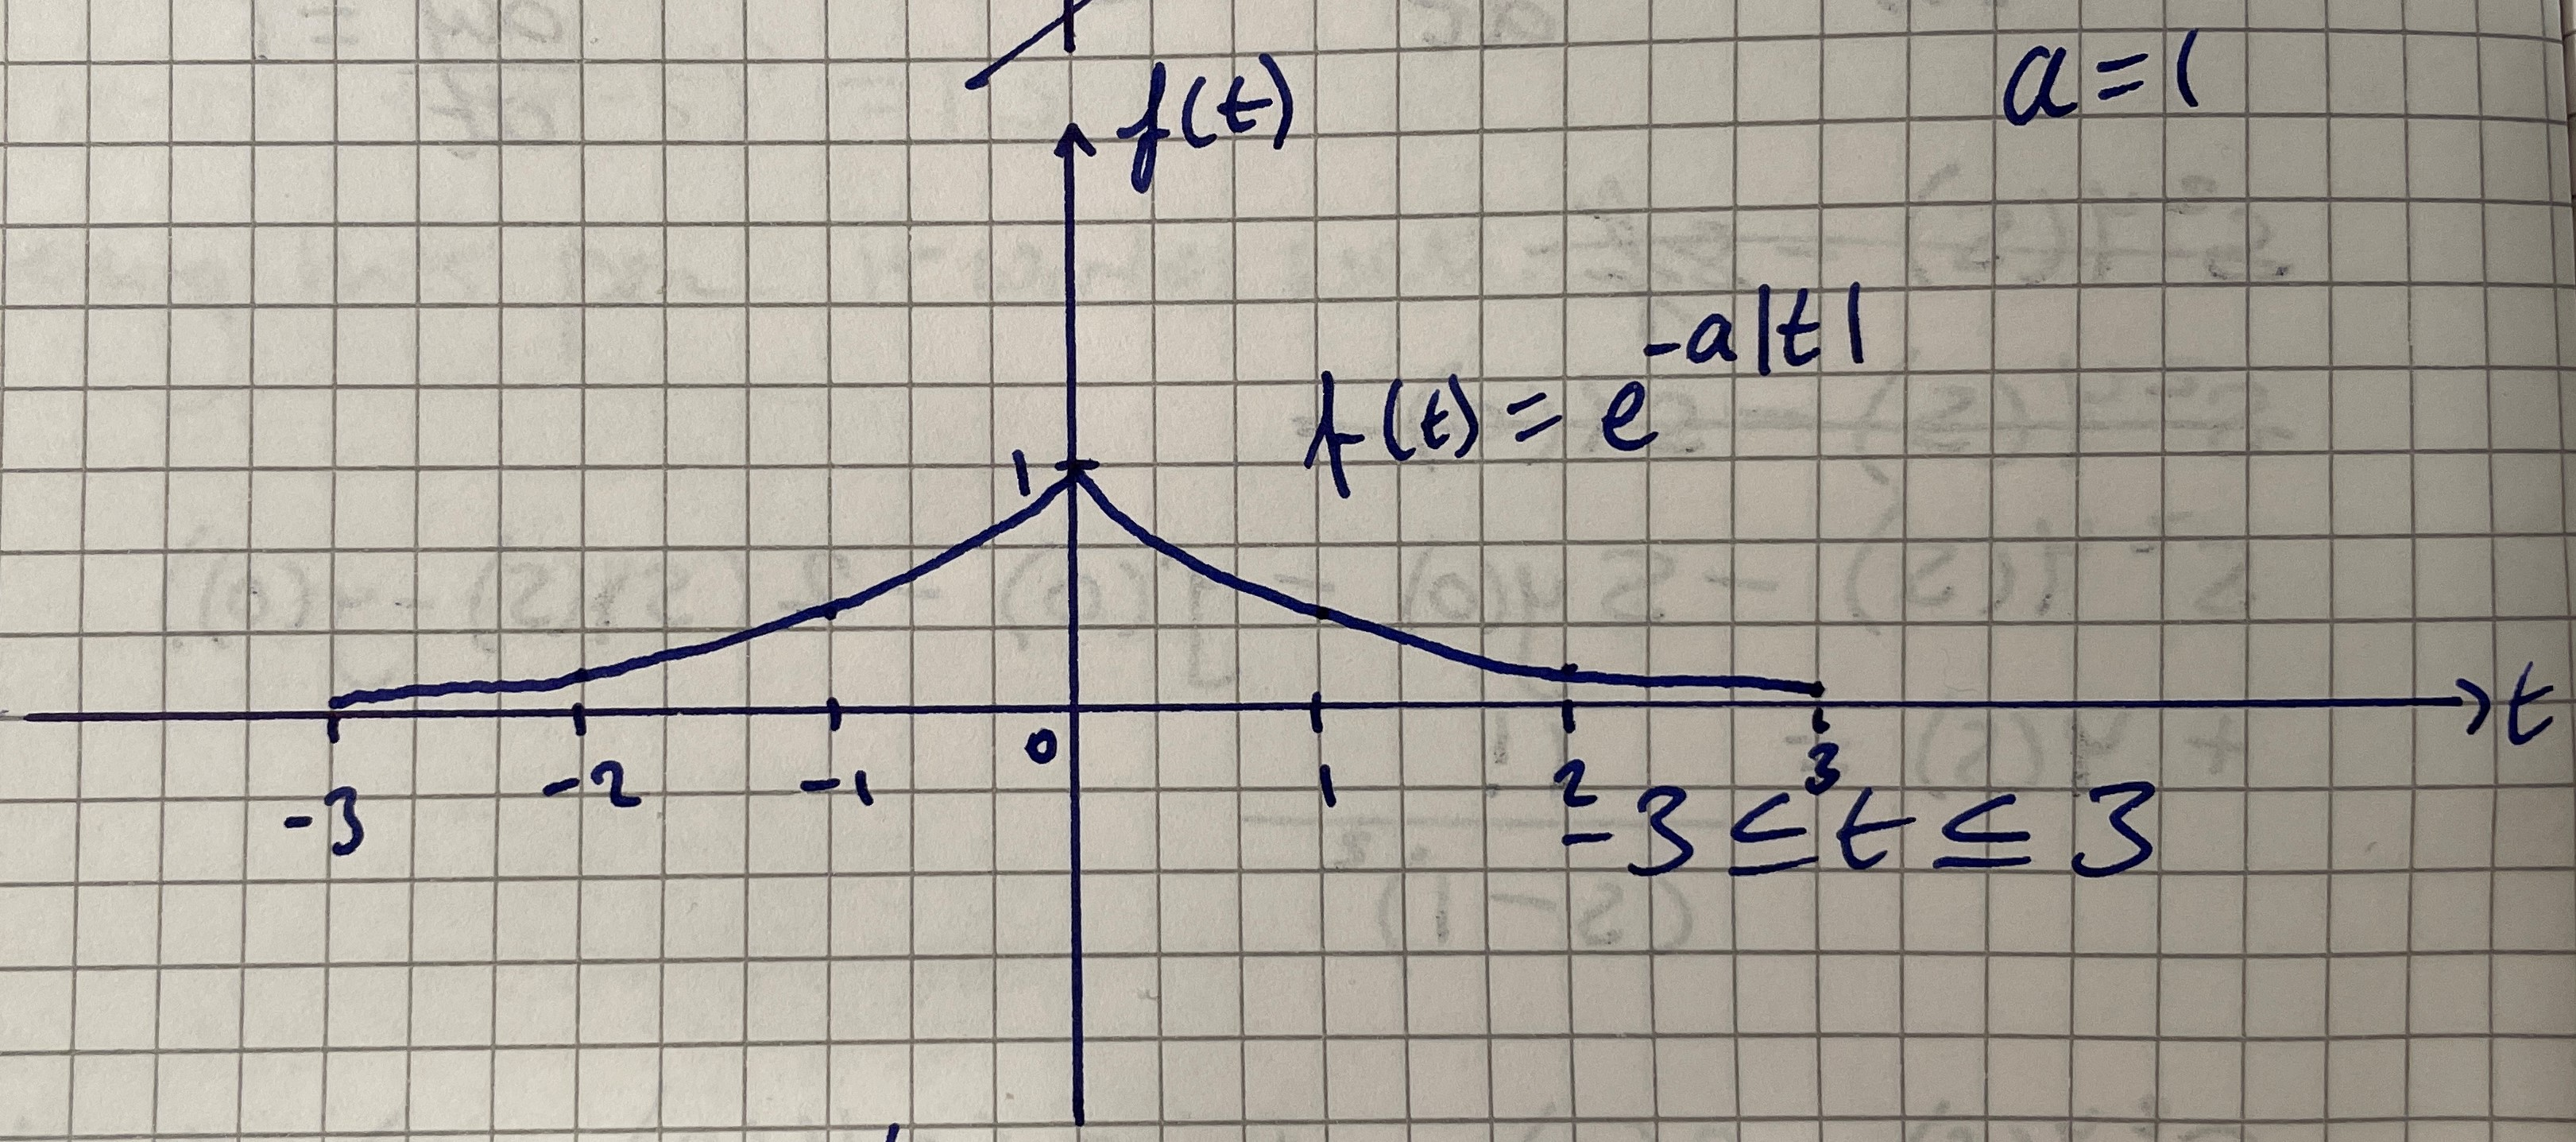
\includegraphics[width = 0.7\textwidth]{./img/q1ei.JPG}
	\caption{}
\end{figure}
\subsubsection*{ii}
Let $z = \infty$.
\begin{align}
	F(u) &= \lim_{z\rightarrow \infty} \int_{t=-z}^{0}e^{at}e^{-j2\pi u t}  \,\dif t + \lim_{z\rightarrow \infty}\int_{t=0}^{z} e^{-at} e^{-j2\pi u t}\,\dif t\\
	&= \lim_{z\rightarrow \infty} \int_{t=-\infty}^{0}e^{t(a - j2\pi u)}  \,\dif t + \lim_{z\rightarrow \infty} \int_{t=0}^{\infty} e^{-t(a + j2\pi u)}\,\dif t\\
	F(u) &= \lim_{z\rightarrow \infty} \left[ \left. \frac{1}{\left(a - j2\pi u\right)}e^{t\left(a - j2\pi u\right)} \right|_{t = -z}^0 \right] + \lim_{z\rightarrow \infty} \left[ \left. \frac{1}{-\left(a + j2\pi u\right)}e^{-t\left(a + j2\pi u\right)} \right|_{t=0}^z \right]
\end{align}
Applying limits:
\begin{align}
	\lim_{z\rightarrow \infty} \left[ \frac{1}{\left(a - j2\pi u\right)} \left[ 1 - e^{-z\left(a - j2\pi u\right)} \right] \right] = \left[ \frac{1}{\left(a - j2\pi u\right)} \left[ 1 - 0 \right] \right] &= \frac{1}{a - j2\pi u}\\
	\lim_{z\rightarrow \infty} \left[ \frac{-1}{\left(a + j2\pi u\right)} \left[ e^{-z\left( a + j2\pi u\right)} -1 \right]\right] = \left[ \frac{-1}{\left(a + j2\pi u\right)} \left[ 0 -1 \right]\right] &= \frac{1}{a + j2\pi u}
\end{align}
\begin{align}
	F(u) &= \frac{1}{a - j2\pi u} + \frac{1}{a + j2\pi u}\\
	&= \frac{a + j2\pi u + a - j2\pi u}{a^2 + 4\pi^2 u^2}\\
	F(u) &= \frac{2a}{a^2 + 4\pi^2u^2}
\end{align}
\subsubsection*{iii}
Substituting $\omega = 2\pi u$, $\omega^2 = 4\pi^2 u^2$:
\begin{align}
	F(\omega) = \frac{2a}{a^2 + \omega^2}
\end{align}
\begin{figure}[H]
	\centering
	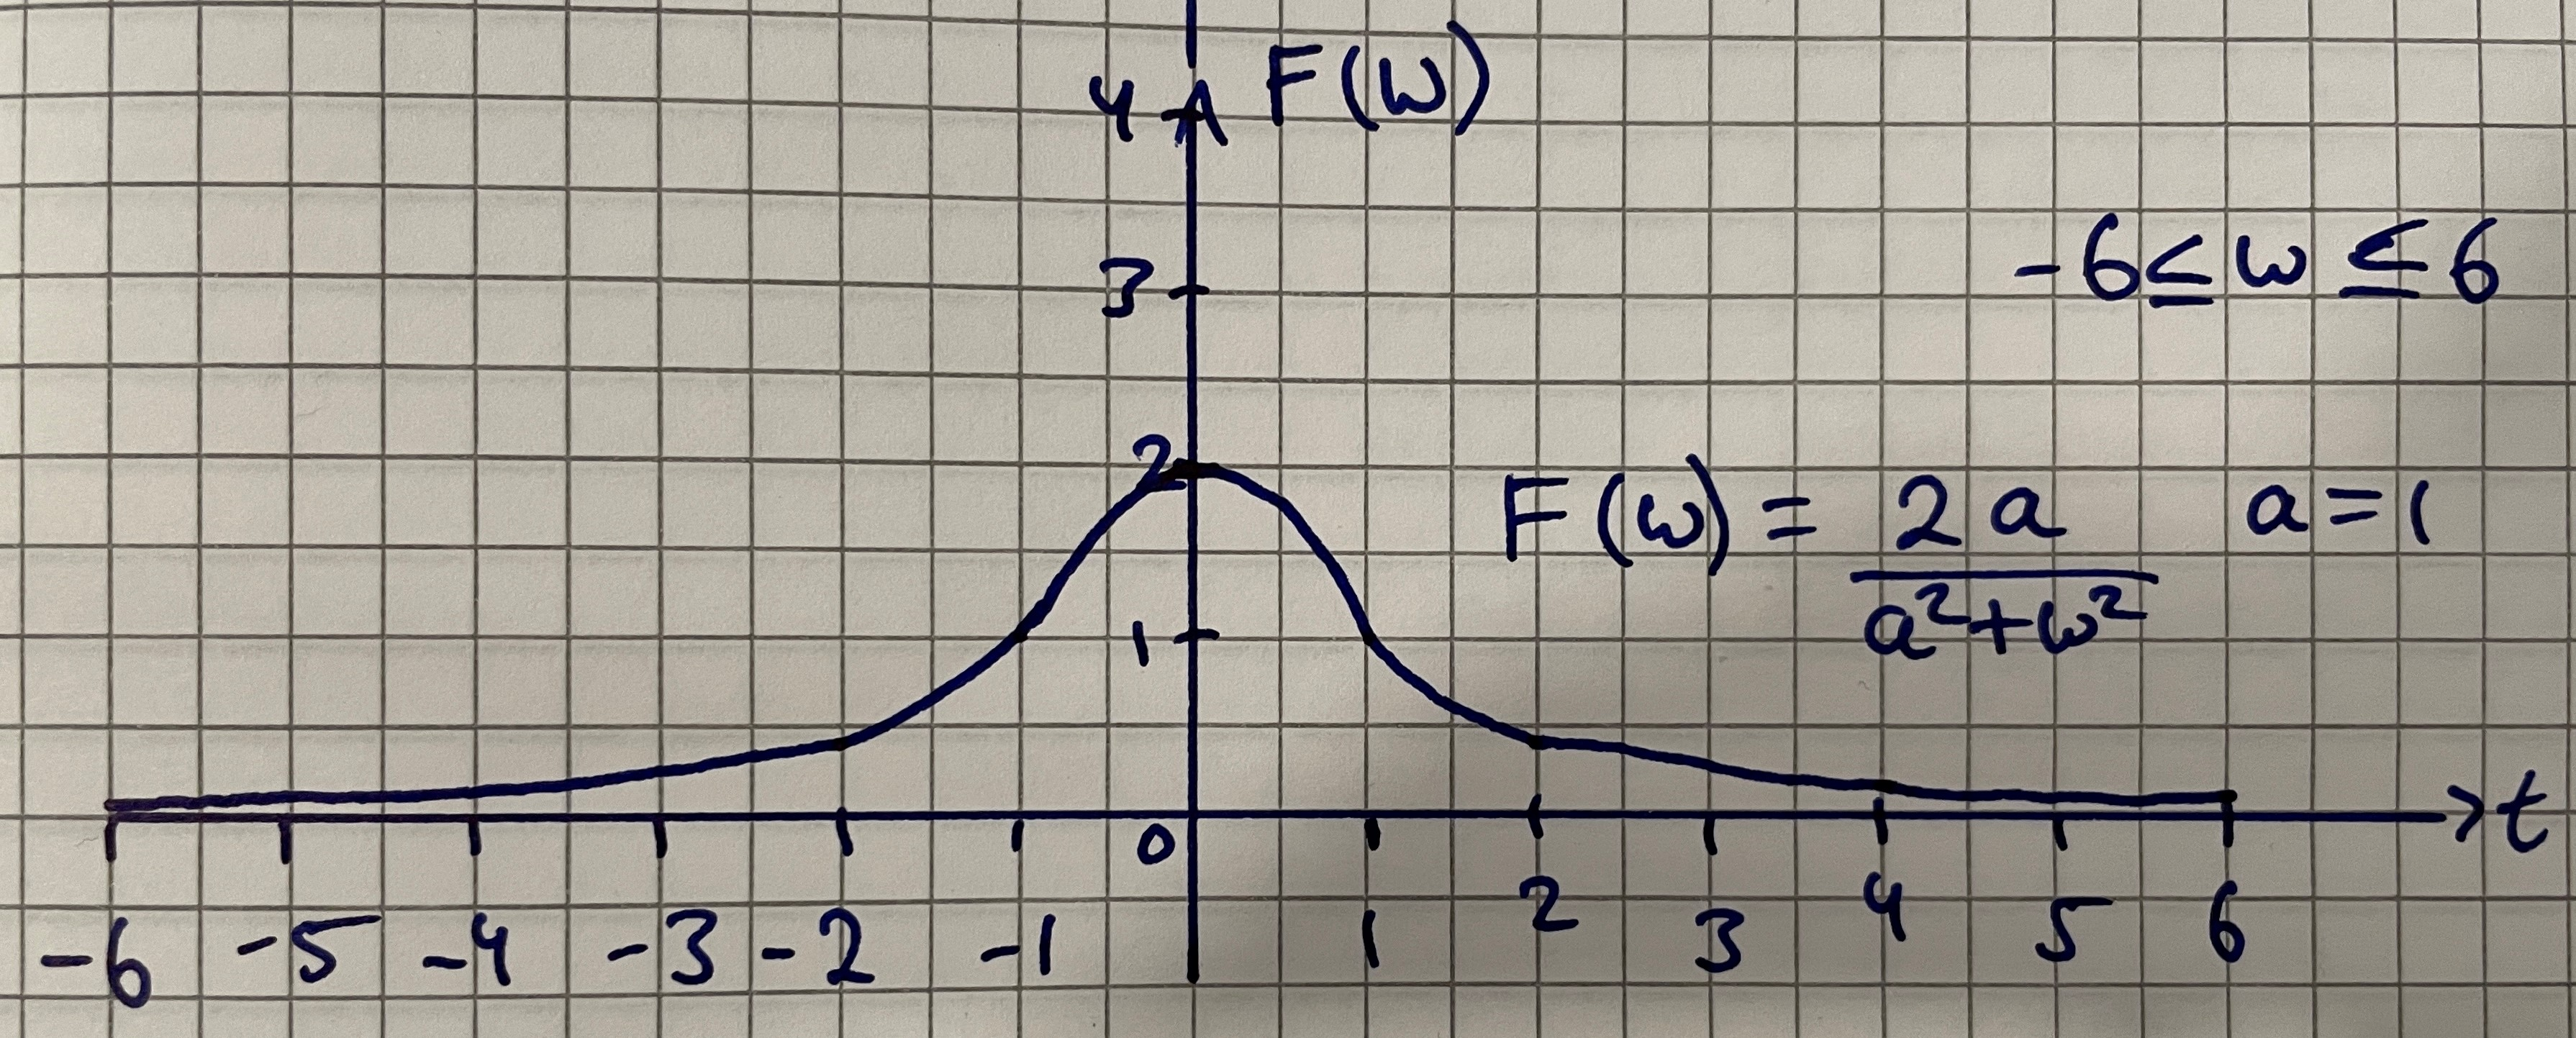
\includegraphics[width = 0.7\textwidth]{./img/q1eiii.JPG}
	\caption{}
\end{figure}
\subsubsection*{iv}
Full width at half maximum of $F\left(u\right)$ can be calculated as:
\begin{align}
	\frac{1}{2} &= e^{-at}\\
	\ln \left(\frac{1}{2}\right) &= -at\\
	-\ln \left(2\right) &= at\\
	t &= \frac{\ln \left( 2 \right)}{a} \rightarrow \textrm{HWHM}\\
	\therefore t &= \frac{2\ln \left( 2 \right)}{a} \rightarrow \textrm{FWHM}
\end{align}
Full width at half maximum of $F\left(\omega\right)$ can be calculated as:
\begin{align}
	\frac{1}{2}\cdot\frac{2}{a} &= 2\frac{a}{a^2 + \omega^2}\\
	\frac{1}{a} &= \frac{2a}{a^2 + \omega^2}\\
	\omega^2 + a^2 &= 2a^2\\
	\omega &= a \rightarrow \textrm{HWHM}\\
	\therefore \omega &= 2a \rightarrow \textrm{FWHM}
\end{align}
\subsubsection*{v}
Product of FWHMs:
\begin{align}
	2a\cdot \frac{2\ln\left(2\right)}{a} &= 4\ln\left(2\right)
\end{align}
The product has no $a$ term, thus there is no dependence on the parameter.
\section{Question Two}
\subsection*{a}
\subsubsection*{i}
\begin{align}
	\frac{\partial u}{\partial t} = k \frac{\partial^2 u}{\partial x^2}\label{PDEq2ai}
\end{align}
We know that $u(x,t) = X(x)T(t)$. Substituting:
\begin{gather}
	X\left(x\right) T'\left(t\right) = kX''\left(x\right)T\left(t\right)\\
	\frac{T'\left(t\right)}{kT'\left(t\right)} = \frac{X''\left(x\right)}{X\left(x\right)} = -\mu \\
	-X''\left(x\right) = \mu X\left(x\right)\\
	T'\left(t\right) = -\mu k T\left(t\right)
\end{gather}
where $\mu$ is an arbitrary constant. 
\subsubsection*{ii}
$\mu$ can be either positive, zero or negative. Let us consider these cases. 

\textbf{Case 1: positive $\mu = \lambda^2 > 0$}
\begin{align}
	\frac{X''\left(x\right)}{X\left(x\right)} &= \lambda^2\\
	X''\left(x\right) - \lambda^2X\left(x\right) &= 0 
\end{align}
Auxiliary equation:
\begin{gather}
	m^2 - \lambda^2 = 0\\
	m_1 = \lambda, \ m_2 = -\lambda
\end{gather}
Real and distinct roots. Hence:
\begin{align}
	X(x) = Ae^{\lambda x} + Be^{-\lambda x}
\end{align}
Applying boundary conditions for $x$. Applying $u\left(0,t\right) = 0$ implies $X(0)T(t) = 0$. Substituting $x=0$ in $X(x)$ gives:
\begin{gather}
	X(0) = A + B\\
	\left(A+B\right)T(t) = 0\\
	T(t) = 0 \textrm{ or } A + B =0
\end{gather}
$T(t) = 0$ leads to a trivial solution of $u(x,t) = X(x)T(t) = 0$. We also have $A + B = 0$ or $A = - B$:
\begin{gather}
	X(x) = A\left(e^{\lambda x} - e^{-\lambda x}\right)
\end{gather}
Applying $u(l,t) = 0$ implies $X(l)T(t) = 0$. Substituting $x=l$ in $X(x)$ gives: $X(l) = A\left(e^{\lambda l} - e^{-\lambda l}\right)$
\begin{gather}
	A\left(e^{\lambda l} - e^{-\lambda l}\right)T(t) = 0\\
	A = 0, \ T(t) = 0, \textrm{ or } e^{\lambda l} - e^{-\lambda l} = 0
\end{gather}
$T(t) = 0$ and $A=0$ both will lead to a trivial solution of $u(x,t) = X(x)T(t) =0$. $e^{\lambda l} - e^{-\lambda l} = 0$ is only true if $\lambda = 0$. However, the assumption in this case is $\lambda = \sqrt{\mu}$ where $\mu$ is a positive constant ($\lambda > 0$). Therefore, this boundary condition cannot be met and there are no useful solutions from Case 1.

\textbf{Case 2: zero constant $\lambda = 0$}
\begin{gather}
	\frac{X''(x)}{X(x)} = \lambda = 0\\
	X''(x) = 0\\
	\int X''(x) \dif x = \int \dif x\\
	X'(x) = C\\
	\int X'(x) = \int C \dif x\\
	X(x) = Cx + D
\end{gather}
where $C$ and $D$ are constants of integration. Applying boundary conditions for $x$. Applying $u(0,t) = 0$ implies $X(0)T(t) = 0$. Substituting $x=0$ in $X(x)$ gives:
\begin{gather}
	X(0) = D\\
	DT(t) = 0
	T(t) = 0 \textrm{ or } D = 0
\end{gather}
$T(t) = 0$ will lead to a trivial solution of $u(x,t) = X(x)T(t) =0$. Therefore, $D=0$.
\begin{align}
	X(x) = Cx
\end{align}
Applying $u(l,t) = 0$ implies $X(l)X(t) = 0$. Substituting $x=l$ in $X(x)$ gives:
\begin{gather}
	X(l) = Cl\\
	ClT(t) = 0\\
	T(t) = 0 \textrm{ or } C = 0
\end{gather}
$T(t) = 0$ and $C=0$ both will lead to a trivial solution of $u(x,t) = X(x)T(t) =0$. Case 2 only produces the trivial solution of $u(x,t) = X(x)T(t) =0$ and does not produce any useful solutions. 
\subsubsection*{iii}
Using Fourier series:
\begin{align}
	c_n = \frac{2}{l}\int_{0}^{l} \left(f(x)\sin\left(n\pi x\right)\right) \,\dif x 
\end{align}
We are given:
\begin{align}
	u(x,0) = f(x) = x^2, \ 0 \leq x \leq l\\
	u(0,t) = u(l,t) = 0, \ t > 0\\
\end{align}
Let $a = \frac{n\pi}{l}$. Substituting the above into Fourier:
\begin{align}
	c_n = \frac{2}{l} \int_{0}^{l} \left( x^2 \sin\left(a x\right) \right) \,\dif x \\
\end{align}
Integration by parts once. $u = x^2$, $u' = 2x$, $v = -\frac{\cos\left(a x\right)}{n\pi}$ and $v' = \sin\left(a x\right)$.
\begin{align}
	c_n = \frac{2}{l}\left[ -\frac{x^2 \cos\left(a x\right)}{a} + \frac{2}{a}\int_{0}^{l} \left(x\cos\left(a x\right)\right) \,\dif x \right]_0^l
\end{align} 
Integration by parts twice. $u = x$, $u = 1$, $v= \frac{\sin\left(a x\right)}{a}$ and $v' = \cos\left(a x\right)$.
\begin{align}
	c_n &= \frac{2}{l}\left[ -\frac{x^2 \cos\left(a x\right)}{a} + \frac{2}{a}\left[ \frac{x\sin\left(a x\right)}{a} - \frac{1}{a} \int_{0}^{l} \left(\sin\left(a x\right)\right) \,\dif x \right]_0^l \right]_0^l\\
	&= 2\left[ -\frac{x^2 \cos\left(n\pi x\right)}{n\pi} + \frac{2}{n\pi}\left[ \frac{x\sin\left(n\pi x\right)}{n\pi} - \frac{1}{n\pi} \left[ -\frac{\cos\left(n\pi x\right)}{n\pi} \right] \right]_0^l \right]_0^l\\
	&= \frac{2}{l}\left[ -\frac{x^2 \cos\left(a x\right)}{n\pi} + \frac{2x\sin\left(a x\right)}{a^2} + \frac{2\cos\left(a x\right)}{a^3} \right]_0^l\\
	&= \frac{2}{l}\left[ -\frac{l^3 \cos\left(n\pi x\right)}{n\pi} + \frac{2l^3\sin\left(n\pi x\right)}{n^2\pi^2} + \frac{2l^3\cos\left(n\pi x\right)}{n^3\pi^3} \right]_0^l\\
	&= \frac{2l^2}{n\pi}\left[ -\cos\left(n\pi x\right) + \frac{2\sin\left(n\pi x\right)}{n\pi} + \frac{2\cos\left(n\pi x\right)}{n^2\pi^2} \right]_0^l\\
	c_n &= \frac{2l^2}{n\pi}\left[ -\cos\left(n\pi\right) + \frac{2\sin\left(n\pi\right)}{n\pi} +\frac{2\left(\cos\left(n\pi\right)-1\right)}{n^2\pi^2} \right]
\end{align}
Substituting:
\begin{align}
	\therefore u_n \left(x,t\right) = \sum_{n=1}^{\infty} \left(\frac{2l^2}{n\pi}\left[ -\cos\left(n\pi\right) + \frac{2\sin\left(n\pi\right)}{n\pi} +\frac{2\left(\cos\left(n\pi\right)-1\right)}{n^2\pi^2} \right] \cdot \sin\left(\frac{n\pi x}{l}\right) \cdot e^{\frac{n^2\pi^2}{l^2}kt} \right)
\end{align}
When $n$ is even:
\begin{align}
	u_n \left(x,t\right) = \sum_{n=1}^{\infty} \left( -\frac{2l^2}{n\pi} \cdot \sin\left(\frac{n\pi x}{l}\right) \cdot e^{\frac{n^2\pi^2}{l^2}kt} \right)
\end{align}
When $n$ is odd:
\begin{align}
	u_n \left(x,t\right) = \sum_{n=1}^{\infty} \left( -\frac{2l^2}{n\pi}\left[1 - \frac{4}{n^2\pi^2}\right] \cdot \sin\left(\frac{n\pi x}{l}\right) \cdot e^{\frac{n^2\pi^2}{l^2}kt} \right)
\end{align}
\subsection*{b}
\subsubsection*{i}
\subsubsection*{ii}
\subsubsection*{iii}
\subsubsection*{iv}
\subsubsection*{v}
\section{EXTRA STUFF}
\subsection*{q2aii}
Where $\mu$ is the eigenvalue. Returning to our PDE in Eq.\ref{PDEq2ai}, if $u_1$ and $u_2$ are solutions to the PDE, so are $C_1 u_1$ and $C_2 u_2$:
\begin{align}
	\frac{\partial C_1 u_1}{\partial t} &= k\frac{\partial^2 C_1 u_1}{\partial x^2}\\
	\frac{\partial u_1}{\partial t} &= k\frac{\partial^2 u_1}{\partial x^2}
\end{align}
Similarly $C_1 u_1 + C_2 u_2$ will satisfy the PDE:
\begin{align}
	U = C_1 u_1 + C_2 u_2 + ... + C_n u_n
\end{align}
We can also form the following equation:
\begin{align}
	A\underline{X} = \mu \underline{X}
\end{align}
Where $A = n \times n$ matrix, $\underline{X} = n \times 1$ column vector and $\mu$ is a scalar. 
\begin{align}
	A \underline{X} - \mu \underline{X} &= 0\\
	\left( A - \mu I\right)\underline{X} &= 0
\end{align} 
We have:
\begin{align}
	\det \left(A - \mu I\right)\underline{X} &= 0\\
	\left| A - \mu I \right| &= 0
\end{align}
Where $\underline{X}$ is the eigenvector.

\begin{align}
	X''(x) + \mu X(x) &= 0\\
	\textrm{Let } X(x) &= e^{mx}\\
	X'(x) &= me^{mx}\\
	X''(x) &= m^2e^{mx}\\
	m^2 + \mu &= 0\\
	m &= \pm j\sqrt{\mu}\\
\end{align}
General solution:
\begin{align}
	X(x) = A\cos\left(\sqrt{\mu}x\right) + B\sin\left(\sqrt{\mu}x\right)
\end{align}
Boundary conditions:
\begin{align}
	u\left(0,t\right) &= 0\\
	X(0)T(t) &= 0\\
\end{align}
We require that $X(0) = 0$. Hence:
\begin{align}
	X(0) &= A\cos\left(0\right) + B\sin\left(0\right)\\
	\therefore A &= 0\\
	X(x) &= B \sin\left(\sqrt{\mu}x\right)\\
	u\left(l,t\right) &= 0\\
	X(l) &= B\sin\left(\sqrt{\mu}l\right) = 0\\
	\sqrt{\mu}l &= n\pi \textrm{ where } n = 1, \ 2, \ 3, \ ... \\
	\mu &= \frac{n^2 \pi^2}{l^2}
\end{align}
Returning to Eq.\ref{TPDE}:
\begin{align}
	\frac{\dif T}{\dif t} &= -k\mu T\\
	\int_{}^{} \left(\frac{1}{T}\frac{\dif T}{\dif t}\right) \,\dif t &= -k\mu \int_{}^{}  \,\dif t\\
	\ln T &= -k \mu t + \ln B\\
	\ln \left(\frac{T}{B}\right) &= - k\mu t\\
	\frac{T}{B} &= e^{--k\mu t}\\
	T &= Be^{-k\mu t}, \ \mu = \frac{n^2 \pi^2}{l^2} \\
	\therefore T &= Be^{-k \frac{n^2 \pi^2}{l^2}t} 
\end{align}
$u(x,t) = X(x)T(t)$. Hence, by utilising principle of superposition:
\begin{align}
	u_n(x,t) = \sum_{n=1}^{\infty} c_n \sin\left(\frac{n\pi}{l}x\right)e^{-k \frac{n^2 \pi^2}{l^2}t}
\end{align}
We are given that $u(x, 0) = f(x)$. Hence, $f(x)$ is:
\begin{align}
	u(x,0) = f(x) = \sum_{n=1}^{\infty} c_n \sin\left(\frac{n\pi}{l}x\right)
\end{align}
\end{document}